\section{Laitossuunnitteluohjelmistoon optimoitu tietorakenne} \label{mun}

Tässä luvussa esitellään pistepilvien käsittelyyn ja visualisointiin soveltuva tietorakenne ja algoritmeja erityisesti laitossuunnitteluohjelmiston tarpeisiin. Ensin määritellään vaatimukset tietorakenteelle tyypillisten pistepilvien käyttötapausten mukaan, jonka jälkeen valitaan alan kirjallisuudesta sovelluskohteelle hyödyllisimmät tekniikat.

\subsection{Käyttötapaukset ja vaatimukset tietorakenteelle}\label{usecase}

Kolme yleistä käyttötapausta pistepilvien kanssa työskenneltäessä ovat mallintaminen, mittaaminen ja katselu, jotka asettavat erilaisia vaatimuksia pistepilviä käsittelevälle ja visualisoivalle laitossuunnitteluohjelmistolle. Esitellään seuraavaksi käyttötapaukset ja niiden asettamat vaatimukset. 

\subsubsection{Mallintaminen}
 Kun laitoksesta halutaan luoda ajantasalla oleva 3d-malli pistepilven avulla, täytyy se mallintaa suunnitteluohjelmiston käyttämäksi geometriaksi pistepilveä mukaillen. Lattiat ja seinät on tasoina helppo asettaa paikalleen, kuten myös suunnitteluohjelmiston komponenttikirjastosta löytyvät laitteet. Suurin työ on yleensä putkistoissa, ilmakanavissa ja kaapeliradoissa. Useat suunnitteluohjelmistot tarjoavat jonkinasteista automatisointia etenkin putkien reititykseen pistepilven päälle. Ohjelmisto voi automaattisesti tunnistaa pilvestä sylintereitä ja asettaa niiden päälle sopivia putkisto-osia. Vaihtoehtoisesti käyttäjä voi valita pilvestä muutamia pisteitä ja ohjelmisto laskee niiden perusteella putken pituuden ja halkaisijan ja asettaa oikean osan paikalleen. Mallinnustyö ja etenkin automaattiset muodontunnistusalgoritmit asettavat ohjelmistolle vaatimuksen tarkkuudesta. Laitossuunnitteluohjelmistossa käytetään yleensä millimetrejä perusyksikköinä, joten pistepilvessä ei saisi esiintyä senttimetrien virheitä.

Mallintamisessa tärkeässä roolissa on suunnittelijan käyttämät näkymät ja pistepiven rajaaminen. Yleensä suunnittelija käyttää muutamaa koordinaattiakselien suuntaista näkymää samanaikaisesti, jotta kursorin saa helposti oikeaan paikkaan. Näkymän syvyys asetetaan usein hyvin pieneksi, jotta mallista näkyisi vain kulloisenkin mallinnustyön vaatima pieni siivu. Myös pistepilveä voidaan rajata niin, että siitä näkyy vain tarpeellinen osa. Pistepilviä visualisoivan ohjelmiston tulisi siis kyetä rajaamaan pilveä toistuvasti ja nopeasti. Käyttökokemus olisi paras, jos käyttäjä pystyisi hiirellä interaktiivisesti määrittämään tilan, jonka sisäpuolella olevat pisteet renderöitäisiin. Lisäksi pistepilvi tulee voida renderöidä useaan eri näkymään samanaikaisesti.

\subsubsection{Mittaaminen}
Toinen tärkeä ominaisuus pistepilvien kanssa työskennellessä on mittaaminen. Pistepilviä käytetään usein tarkastamaan, mahtuuko laitokseen jokin uusi laite tai putkisto. Tällöin on hyödyllistä suorittaa mittauksia joko kahden pistepilven pisteen, tai pisteen ja 3d-mallin geometrian välillä. Mittausoperaatiossa käyttäjä valitsee pistepilvestä kursorilla haluamansa pisteen ja ohjelmisto palauttaa lähimmäksi kursoria projisoidun pisteen. Käyttäjän kannalta olisi miellyttävää, jos mittausoperaatioita tehtäessä ei tarvitsisi odottaa, kun pistepilven miljoonien pisteiden joukosta etsitään juuri kursorin alla oleva piste. Yksittäisten pisteiden hakeminen pilvestä täytyy siis olla nopeaa.

\subsubsection{Katselu}
Kolmas yleinen pistepilvien käyttökohde on 3d-mallin katselu joko laitossuunnitteluohjelmistossa tai erityisessä mallinkatseluohjelmistossa. Etenkin suunnitteluprojektien esimiehet haluavat usein tarkastella suunnittelijoiden luomaa 3d-mallia helposti ja nopeasti. Luonnollisesti malliin kuuluvat pistepilvet tulevat myös näkyä katselijalle. Tämä saattaa tuottaa haasteita ohjelmiston kannalta, sillä katseluohjelmistojen käyttäjillä on käytettävissä harvoin yhtä järeää laitteistoa, kuin suunnittelijoiden työasemat. Mallinkatseluohjelmistossa pistepilveä harvemmin rajataan pienemmäksi, joten renderöitäviä pisteitä on niin paljon, etteivät ne mahdu kerralla keskusmuistiin tai näytönohjaimen muistiin. Yleensä käyttäjä myös liikuttaa näkymää mallin ympäri enemmän kuin mallinnustyössä, joten pistepilvivisualisoinnin suorituskyky ja tarkkuustasot ovat entistäkin tärkeämpiä.

Tässä tutkielmassa kehitetään laitossuunnitteluohjelmistolle optimoitu hierarkinen tietorakenne pistepilvien käsittelyyn. Esitetään tietorakenteelle seuraavat vaatimukset edellä mainittujen käyttötapausten perusteella:
\begin{enumerate}
    \item \label{vaatimus:lod} On voitava visualisoida karkea yleiskuva pistepilvestä vain pienellä osalla datasta. 
    \item \label{vaatimus:ooc} On käytettävä ulkoisen muistin algoritmeja, eli koko pilveä ei pidetä kerralla keskusmuistissa.
    \item \label{vaatimus:harvennus} Pistepilven vaatimaa tallennustilan määrää voidaan laskea harventamalla sen tiheästi näytteistettyjä osia. 
    \item \label{vaatimus:crop} Käyttäjän on voitava määrittää pilvestä alueita, joiden sisältävien tai ulkopuolelle jäävien pisteiden ominaisuuksia, kuten näkyvyyttä tai väriä, voidaan muuttaa.
    \item \label{vaatimus:select} Pilvestä on voitava nopeasti ja tarkasti valita yksittäisiä pisteitä.
    \item \label{vaatimus:virhe} Pistepilvessä ei saa esiintyä yli millimetrin suuruisia virheitä.
\end{enumerate}


\subsection{Tietorakenteen valinta}

Luvussa \ref{tietorakenteet} esitelty Potree on osoittaunut massiivisten pistepilvien interaktiivisen visualisoinnin olevan mahdollista jopa verkkoselaimessa, jossa etenkin tiedonsiirtonopeus rajoittaa renderöinnin nopeutta. Tarkastellaan siis sisäkkäispistepuiden sovelutuvuutta laitossuunnitteluohjelmistoon. 

Oktettipuun läpikäyminen taso kerrallaan muodostaa tehokkaasti tarkkuustasot, joten vaatimus \ref{vaatimus:lod} on helppo tyydyttää. Pisteiden asettelu sisäkkäisten oktettipuiden solmuihin mahdollistaa myös vaatimuksen \ref{vaatimus:ooc} mukaisesti ulkoisen muistin käyttämisen. Scheiblauerin muokattavien sisäkkäisten oktettipuiden jokainen solmu sisältää ruudukon, johon pisteet sijoitetaan. Mitä syvemmällä tasolla solmu on, sitä pienempiä ruudukon solut ovat. Vaatimuksen \ref{vaatimus:harvennus} esittämä pilven harvennus onnistuu asettamalla puulle enimmäissyvyys ruudukon koon mukaan ja hylkäämällä lehtisolmuissa kaikki pisteet, jotka tulisi lisätyksi jo varattuun soluun. 

Valintaoperaatiot onnistuvat nopeasti oktettipuussa. Puun jokainen solmu sisältää tiedon sen sisältämien pisteiden rajauslaatikosta \engl{bounding box}, joten jos valinnan sijainti ei osu rajauslaatikon sisälle, ei kyseisen solmun lapsisolmujakaan tarvitse tarkastaa. Yksittäisiä pisteitä tarvitsee tarkastella vasta kun valittavan alueen raja kulkee puun solmun rajauslaatikon läpi, tai kun käyttäjä haluaa valita vain yhden pisteen. Tietyllä aluella sijaitsevat pisteet jakautuvat useaan oktettipuun solmuun, minkä johdosta valintaoperaatiot eivät ole triviaaleja sisäkkäisissä oktettipuissa. Vaatimuksiin \ref{vaatimus:crop} ja \ref{vaatimus:select} voidaan kuitenkin vastata sisäkkäisillä oktettipuilla. Scheiblauer ja Schütz eivät tiivistäneet pistepilviä, joten niiden tarkkuus ei kärsinyt. Näin myöskään vaatimus \ref{vaatimus:virhe} ei tuota ongelmia.

Sisäkkäispistepuut näyttävät siis soveltuvan myös laitossuunnitteluohjelmiston tarpeisiin. Scheiblauerin ja Schützin tietorakenteiden käyttämät ruudukot mahdollistavat kuitenkin myös joitakin laitossuunnittelusovelluksille tärkeitä optiomointeja. Esitellään seuraavaksi, miten pistedataa voi tiivistää ruudukon avulla.


\subsection{Pistedatan esitysmuoto}\label{kompressio}

Pistepilvet sisältävät usein satoja miljoonia tai jopa miljardeja pisteitä, mikä johtaa luonnollisesti isoihin tiedostokokoihin. Yleensä hierarkiatiedon osuus tiedoston sisällöstä on varsin pieni, joten tiedostokokoa saadaan pienennettyä parhaiten tiivistämällä itse pisteiden esitysmuotoa. Pisteistä tarvitsee tallentaa vähintään niiden sijainti ja väri. Yleensä sijainti esitetään kolmella nelitavuisella liukuluvuilla ja väri RGB-koodauksella kolmella yksitavuisella kokonaisluvulla:

\code{
struct Point \{\\
    \tab float x;\\
    \tab float y;\\
    \tab float z;\\
    \tab unsigned char r;\\
    \tab unsigned char g;\\
    \tab unsigned char b;\\
    \}
}

\noindent Yleensä näiden 15:a tavun lisäksi lisätään yksi pakkaustavu, jotta koko olisi mukava kahden potenssi. Miljardi pistettä tallennettuna tässä esitysmuodossa vaatisi siis 16 gigatavua muistia.\footnote{Pistepilvisovelluksen käyttäjän rahapussin koosta riippuen tämän kokoinen pilvi mahtuisi vielä keskusmuistiin ja jopa näytönohjaimen muistiin \cite{rtx}.} Muuttamalla pisteiden esitysmuotoa voidaan pistepilviä tiivistää ja joitakin operaatioita nopeuttaa.

\begin{figure}
    \subfile{fig/ruudukko.tex}
    \caption{64:n solun ruudukko, jonka indeksointi alkaa vasemmasta alakulmasta}
    \label{ruudukkokuva}
\end{figure}

Sisäkkäispistepuiden käyttämä ruudukko mahdollistaa yksinkertaisen pakkausalgoritmin. Puun rakennusvaiheessa pisteet lisätään jokaisessa solmussa olevaan kolmiulotteiseen ruudukkoon, jonka jokaiseen soluun mahtuu vain yksi piste. Kun piste lisätään ruudukon soluun, tallennetaan solun järjestysnumero hajautustauluun, josta voidaan jatkossa nopeasti tarkastaa, onko kyseinen solu varattu. Mahdollinen numerointi ruudukolle on esitetty kuvassa \ref{ruudukkokuva}. Numerointi alkaa vasemmasta alakulmasta indeksistä nolla ja etenee vasenkätisen koordinaatiston mukaisesti. 

Puun solmuihin on tallennettu rajauslaatikko, joka määrittää myös ruudukon mitat ja sijainnin. Ruudukkoon lisättävien pisteiden absoluuttinen sijainti voidaan unohtaa ja käyttää sijainnin tallentamiseen pisteen suhteellista sijaintia ruudukossa. Yksinkertaisimmillaan voidaan kustakin pisteestä tallentaa vain sen solun indeksi, jossa piste sijaitsee. Tällöin pisteen esitysmuoto on siis

\code{
struct Point \{\\
    \tab unsigned int index;\\
    \tab unsigned char r;\\
    \tab unsigned char g;\\
    \tab unsigned char b;\\
    \}
}

\noindent Kun solun indeksi tallennetaan etumerkittömänä nelitavuisena kokonaislukuna ja lisätään loppuun yksi pakkaustavu, tiivistyy piste kahdeksantavuiseksi. Näin miljardi pistettä vaatisi enää 8 gigatavua muistia. 

Esitysmuotoa voidaan tiivistää vielä tästäkin. Pisteen etäisyyttä suhteessa ruudukkoon voidaan esittää kolmella tavulla niin, että jokainen tavu kuvaa koordinaattiakselien suuntaisten askelten määrää ruudusta 0 lähtien. Yhden tavun esittämä enimmäisarvo on 255, joten ruudukossa voi olla enintään $255^3=16581375$ solua. Tällainen kompressio tuo toki pistepilveen epätarkkuutta, johon palataan myöhemmin. %TODO: \ref{error}

Usein laitossuunnittelussa käytetyissä laserkeilaimissa ei käytetä värikameraa antamaan pisteille värejä, vaan väri-informaatio johdetaan keilaimeen heijastuvan valon määrästä. Tämä arvo normalisoidaan yleensä välille $[0,255]$, josta saadaan jokin harmaan sävy. Tällaisissa pistepilvissä on siis turha tallentaa jokaiselle pisteelle \texttt{r}, \texttt{g} ja \texttt{b} -arvoja, kun vain yksi arvo riittäisi. Näin piste voidaan esittää muodossa 

\code{
struct Point \{\\
    \tab unsigned char dx;\\
    \tab unsigned char dy;\\
    \tab unsigned char dz;\\
    \tab unsigned char intensity;\\
    \}
}

\noindent eli tarvitaan vain neljä tavua tilaa ja edellä mainittu pistepilvi saadaan tiivistettyä neljännekseen alkuperäisestä koostaan. 

\begin{figure}
    \centering
    \subfile{fig/error.tex}
    \caption{Suurin mahdollinen ruudukossa esiintyvä virhe $\epsilon$. Kuutio kuvaa ruudukon solua ja asteriski sen visualisointiin käytettävää keskipistettä. Soluun lisätty punainen piste on juuri ja juuri solun sisällä.}
    \label{errorkuva}
\end{figure}

Kun pisteen tarkka sijainti unohdetaan ja se ilmaistaan suhteessa ruudukkoon, syntyy pistepilveen virheitä. Suurinta mahdollista virhettä on havainnollistettu kuvassa \ref{errorkuva}, kun piste visualisoidaan solun keskipisteenä, vaikka se oikeasti sijaitsisi aivan sen nurkassa. Jos oletetaan, että ruudukon solut ovat kuutioita, saadaan enimmäisvirhe laskettua helposti Pythagoraan lauseella muotoon 
\begin{equation}
    \epsilon = \frac{a \sqrt{3}}{2}.      
\end{equation}

Vaatimus \ref{vaatimus:virhe} esitti virheen enimmäissuuruudeksi yhtä millimetriä. Oktettipuu jakaa rajauslaatikon sivun kahtia joka tasolla ja ruudukko sen edelleen pieniin soluihin. Jos oletetaan esimerkiksi pistepilven rajauslaatikko kuutioksi, jonka sivun pituus on sata metriä ja ruudukon sisältävän Scheiblauerin ja Schützin käyttämää 128 solua jokaiseen koordinaattiakselin suuntaan, saavutetaan puun tasolla 11 ruudukko, jonka solun sivun pituus on $a = \frac{100m/2^{10}}{128} \approx 0,763mm$. Tällaisessa ruudukossa enimmäisvirhe on $\frac{0,763mm \cdot \sqrt{3}}{2} \approx 0,661mm$, joten kaikki tähän ruudukkoon lisätyt pisteet täyttävät vaatimuksen \ref{vaatimus:virhe}. Tämä ei tarkoita sitä, että puu voisi sisältää pisteitä vain tasolta 11 alaspäin. Pisteitä voi hyväksyä suuriinkin soluihin, jos ne ovat tarpeeksi lähellä sen keskipistettä.

Pisteiden sijainnin suhteellinen esitysmuoto nopeuttaa myös pistepilvien käsittelyä. Laitossuunnittelussa pistepilveä joudutaan usein sovellukseen latauksen jälkeen liikuttamaan ja skaalaamaan, jotta se istuisi hyvin 3d-malliin. Jos pisteisiin olisi tallennettu absoluuttinen sijainti, jouduttaisiin pistepilveä tallennettaessa uudelleenkirjoittamaan kaikki pisteet käyttäjän määrittämällä transformaatiomatriisilla kerrottuna. Edellä kuvatulla esitysmuodolla transformaatio täytyy suorittaa vain oktettipuun solmujen rajauslaatikoilla, joista tiivistetyn pisteen sijainti johdetaan. Tämä johtaa merkittävään parannukseen käyttökokemuksessa, sillä satojen miljoonien pisteiden kirjoittaminen levylle voi kestää kymmeniä minuutteja.

\subsection{Tietorakenteen rakentaminen}

Edellä todettiin sisäkkäispistepuiden sopivan pistepilvien käsittelyyn käytettäväksi tietorakenteeksi laitossuunnitteluohjelmistossa ja ehdotettiin pisteille kompaktimpaa esitysmuotoa. Käydään nyt läpi puun rakentamiseen käytettyjä algoritmeja.

Puun rakentaminen suoritetaan kahdessa vaiheessa. Ensin käydään kaikki syötepisteet läpi ja selvitetään niille rajauslaatikko. Tämän jälkeen luodaan tyhjä juurisolmu, jonka rajauslaatikkona toimii äsken laskettu, kaikki pisteet sisältävä rajauslaatikko. Nyt syötepisteet voidaan lisätä yksitellen juurisolmuun, joka syöttää ne tarvittaessa edelleen lapsisolmuilleen. Rakentamisen ylintä tasoa on kuvattu algoritmissa \ref{alg:rakenna}.

\begin{algorithm}[!h]
    \caption{RakennaOktettipuu}
    \label{alg:rakenna}
    \subfile{alg/rakennapuu.tex}
\end{algorithm}

Algoritmi \ref{alg:lisaaPiste} huolehtii pisteen pisteen lisäämisestä solmuun. Piste hyväksytään solmuun, jos sitä vastaava ruudukon solu on tyhjä, sen etäisyys solun keskipisteestä on pienempi kuin sallittu enimmäisvirhe ja solussa ei ole jo liikaa pisteitä. Solmujen sisältämien pisteiden määrälle kannattaa asettaa yläraja, jotta saavutettaisiin sopiva haarautuminen. Luvussa \ref{render} huomataan, että etenkin puun ylimmillä tasoilla olisi renderöinnin kannalta hyvä, jos solmuissa olisi saman verran pisteitä.

Puun syvyyttä voi rajoittaa asettamalla ruudukon soluille vähimmäismitat. Yleensä laserkeilaimen lähellä olevat pinnat on hyvin tiheästi näytteistettyjä ja tilannetta pahentaa, jos useat keilaimet ovat mitanneet samoja pintoja tiheästi. Algoritmin \ref{alg:lisaaPiste} rivillä 3 tarkastetaan, onko ylittäisikö uusi lapsisolmu puun enimmäissyvyyden. Kun ennaltamäärätylle pohjatasolle hyväksytään kaikki pisteet, kunhan niitä vastaava ruudukon solu on vapaa, saadaan pistepilvelle tehokas ja globaali enimmäistiheys. Tällä tavalla pilveä saadaan harvennettua tehokkaasti ja vaatimus \ref{vaatimus:harvennus} voidaan tyydyttää. %TODO: \ref{arviointi} missä tätä toivottavasti on mitattu

\begin{algorithm}[!h]
    \caption{LisääPisteSolmuun}
    \label{alg:lisaaPiste}
    \subfile{alg/lisaaPiste.tex}
\end{algorithm}

Tietorakennetta tallennettaessa kirjoitetaan tiedostoon ensin tarvittavat tiedot puun solmuista ja pisteet vasta niiden jälkeen. Jokainen solmu sisältää tiedon siitä, kuinka monta pistettä siihen kuuluu, sekä ensimmäisen pisteen indeksin pistetaulukossa. Tämä mahdollistaa sen, että pistepilveä käsiteltäessä luetaan tiedostosta ensin vain kevyt hierarkia, jonka jälkeen vain tarvittavat pisteet voidaan lukea muistiin. Tiedoston rakennetta on havainnollistettu kuvassa \ref{layout}. Pisteiden lukumäärän ja ensimmäisen pisteen indeksin lisäksi jokaisesta solmusta tallennetaan rajauslaatikko ja sijaintikoodi, joka kertoo sen sijainnin puussa. Sijaintikoodin  numerot kertovat reitin juurisolmusta kyseiseen solmuun. Esimerkiksi koodi 014 tarkoittaa juurisolmun toisessa oktetissa sijaitsevan lapsen viidennessä oktetissa sijaitsevaa lasta. Lopuksi tarvitsee levylle kirjoittaa vielä millä puun tasolla se sijaitsee, jotta tiedostoa lukiessa tiedettäisiin sijaintikoodin pituus.

\begin{figure}
    \centering
    \subfile{fig/layout.tex}
    \caption{Tiedostoon tallennetaan ensin puun solmut, joiden jälkeen kaikki pisteet ovat peräkkäin taulukossa. Punaiset nuolet kuvaavat solmuihin tallennettuja indeksejä pistetaulukkoon, josta siihen kuuluvat pisteet alkavat.}
    \label{layout}
\end{figure}

Yksittäinen solmu voidaan siis kirjoittaa levylle muodossa 

\code{
struct Node \{\\
    \tab float min\_x;\\
    \tab float min\_y;\\
    \tab float min\_z;\\
    \tab float max\_x;\\
    \tab float max\_y;\\
    \tab float max\_z;\\
    \tab unsigned char depth;\\
    \tab unsigned char location\_code[];\\
    \tab unsigned int num\_points;\\
    \tab unsigned int point\_index;\\
    \}
}

\noindent Nelitavuisilla liukuluvuilla ja kokonaisluvuilla vaatii solmu siis tallennustilaa $33 + d$ tavua, missä $d$ on solmun syvyys puussa.


\subsection{Renderöinti}\label{render}

Nopein tapa renderöidä pistepilvi on pitää kaikki pisteet näytönohjaimen muistissa ja joka ruudunpäivityksellä piirtää kaikki näkymässä näkyvät pisteet. Vaikka koko pistepilvi mahtuisi näytönohjaimen muistiin, täytyy laitossuunnitteluohjelmistossa visualisoida muutakin grafiikkaa. Näytönohjaimen muistia voidaan säästää käyttämällä niin kutsuttua puskurivirtaa \engl{buffer streaming}. Yleinen ongelma grafiikan renderöinnissä on se, että näytönohjain renderöi dataa nopeammin kuin suoritin ehtii sille syöttää. Puskurivirran ajatuksena on pitää näytönohjain mahdollisimman toimeliaana jakamalla puskuri, jonka kautta dataa siirretään keskusmuistista näytönohjaimen muistiin, kolmeen osaan. Samalla kun näytönohjain käsittelee yhtä puskurin osaa, suoritin voi täyttää toista datalla, ja kolmas on jo palautumassa suorittimen täytettäväksi. Teoriassa näytönohjain voi vain vaihtaa luettavaa puskuria ilman, että sen tarvitsisi odottaa lainkaan hidasta tiedonsiirtoa. \cite{opengl}

\begin{figure}
    \centering
    \subfile{fig/triplebuffering.tex}
    \caption{Pistedatan renderöinnissä käytetty puskuri, joka on jaettu osioihin $b_0$, $b_1$ ja $b_2$. Osioon $b_0$ on kirjoitettu pisteet solmuista $s_0$-$s_3$. Puskurivirran tarkoituksena on vähentää tiedonsiirrosta aiheutuvaa latenssia.}
    \label{triplebuffering}
\end{figure}

Kuvassa \ref{triplebuffering} pistepuskuri on jaettu osioihin $b_0$, $b_1$ ja $b_2$. Puskurin koko on valittu niin, että jokaiseen osioon mahtuu neljän täyden solmun pisteet. Käytännössä solmut eivät kuitenkaan aina ole täysiä, joten on mahdollista, että osiot jäävät vajaiksi. Puskureita kuitenkin vaihdetaan tiuhaan, joten ei ole järkevää käyttää aikaa puskurin täyttöasteen maksimointiin.

Tietorakenteen renderöintiä testatessa puskurivirta ei kuitenkaan tuottanut tarpeeksi miellyttävää visuaalista lopputulosta. Etenkin pilveä pyöriteltäessä ja sen läpi liikuttaessa puskurivirralla ehdittiin pilvestä renderöidä vain hyvin karkea tarkkuus niin, että ruudunpäivitystaajuus pysyi interaktiivisena. Ratkaisuna tähän näytti toimivan hyvin toinen pistepuskuri, jossa säilytetään karkeaa yleiskuvaa pilvestä. Tätä yleiskuvapuskuria päivitetään vain silloin, kun jotkut sen sisältämistä solmuista on pudonnut näkymän ulkopuolelle. 

\begin{algorithm}[!h]
    \caption{RenderöiYleiskuva}
    \label{alg:render}
    \subfile{alg/render.tex}
\end{algorithm}

Algoritmissa \ref{alg:render} yleiskuvapuskuri täytetään ensimmäisellä renderöintikerralla niiden solmujen pisteillä, jotka ovat mahdollisimman ylhäällä puussa, ja ne ovat täynnä, eli sisältävät rakentamisvaiheessa määritellyn enimmäismäärän pisteitä. Seuraavilla renderöintikerroilla puskurista tarkistetaan, ovatko niiden sisältämät pisteet vielä näkyvissä. Jokaista pistettä ei tarvitse tarkastaa, jos ylläpidetään listaa solmuista, joiden pisteet puskuriin lisättiin. Jos näkymä on muuttunut niin, että jokin solmu ei enää ole näkyvissä, vaihdetaan sen pisteet toisen solmun pisteisiin. Yleiskuvapuskurissa pidetään solmuja mahdollisimman läheltä puun juurta, jotta ne muodostaisivat tarpeeksi kattavan kuvan koko pistepilvestä.

\begin{algorithm}[!h]
    \caption{RenderöiPuskurivirta}
    \label{alg:renderDetail}
    \subfile{alg/renderDetail.tex}
\end{algorithm}

Yleiskuvan renderöinnin jälkeen pistepilveä tarkennetaan renderöimällä loput pisteet puskurivirralla. Algoritmi \ref{alg:renderDetail} käy puun solmuja läpi taso kerrallaan ja lisää solmun pisteet täyttövuorossa olevaan puskurivirran osioon, jos solmua ei ole jo renderöity yleiskuvapuskurilla. Puskuriosion täyttyessä vaihdetaan täytettäväksi seuraava osio. Puskurivirrassa täytyy varmistaa, ettei sama osio ole sekä suorittimen kirjoitettavana, että näytönohjaimen luettavana. Tämä tapahtuu lähettämällä näytönohjaimelle jokaisen puskuriosion täyttymisen jälkeen synkronointiobjekti \engl{sync object}. Kun uutta osiota otetaan kirjoitettavaksi, tarkastetaan, että näytönohjain on merkannut kyseisen osion synkronointiobjektin käsitellyksi. \cite{sync}

Algoritmi \ref{alg:renderDetail} suorittaa pistepilvelle näkyvyyskarsintaa \engl{visibility culling}. Puu käydään ensin kokonaan läpi ja renderöitäviksi valitaan vain ne solmut jotka ovat täysin tai osittain näkymäkartion \engl{view frustum} sisällä. Näkyvyyskarsinnan lisäksi algoritmin voidaan katsoa suorittavan yksinkertaista yksityiskohtien karsintaa \engl{detail culling}, kun kuvaruudulle suurena projisoidut solmut renderöidään ensin.

Yksityiskohtien karsinta on suosittu nopeutustekniikka tietokonegrafiikassa. Ajatuksena on renderöidä vain tärkeimmät objektit ja jättää kaukana olevat tai pienet objektit renderöimättä, jotta ruudunpäivitystaajuus pysyy interaktiivisena. Yksinkertainen tapa karsia yksityiskohtia on järjestää objektit niiden kuvaruudulle projisoidun koon mukaan ja renderöidä niitä tiettyyn rajaan asti, tai kunnes aika loppuu kesken. Akenine-Möller et al. \cite{rrr} esittävät kuvaruudulle projisoidun objektin koon arviolle kaavaa 
\begin{equation}
    a = \pi (\frac{nr}{\mathbf{d} \cdot (\mathbf{c}-\mathbf{v})})^2,
\end{equation} jossa $n$ on katselupisteen etäisyys kuvatasosta, $r$ objektin rajauspallon säde ja $\mathbf{c}$ keskipiste, $\mathbf{d}$ on normalisoitu katsomissuunta, ja $\mathbf{v}$ katselupiste. \cite{mikko}

Mikko Yllikäinen huomautti pro gradu -tutkielmassaan \cite{mikko}, ettei tarkkaa arvioita objektien koosta kannata selvittää, jos halutaan selville vain suuruusjärjestys. Yllikäinen yksinkertaistaa kaavan muotoon 
\begin{equation}
    \begin{split}
    a & = \frac{r}{\mathbf{d} \cdot ( \mathbf{c} - \mathbf{v} )}\\
    & \approx \frac{r}{\sqrt{(c_x-v_x)^2 + (c_y-v_y)^2 + (c_z - v_z)^2}}\\
    & \propto \frac{r}{(c_x-v_x)^2 + (c_y-v_y)^2 + (c_z - v_z)^2}.    
    \end{split}
\end{equation}
 Yllikäinen nimittää tällä kaavalla muodostetu suuruusjärjestyksen käyttämistä yksityiskohtien karsinnassa kontribuutiokarsinnaksi \engl{contribution culling}. On huomattava, että tällainen karsinta ei ole mahdollista paralleliprojektiomaisemissa, joissa katseluetäisyys ei vaikuta objektien kokoon. \cite{mikko}


\subsection{Pisteiden valinta}

Yksittäisten pisteiden valinta pistepilvestä on hyvin raskas operaatio, jos pisteet eivät ole hierarkisessa tietorakenteessa. Oktettipuuta käytettäessä kaikkia pisteitä ei tarvitse kuitenkaan käydä läpi. Käyttäjän valitessa hiirellä piste pilvestä ammutaan kamerasta säde kursorin projisoidun sijainnin läpi maisemaan. Nyt pisteitä tarvitsee etsiä vain niistä oktettipuun solmuista, joihin säde osuu. Yksinkertaisimmillaan voidaan valita sädettä lähinnä oleva piste. Tällöin valituksi saattaisi kuitenkin tulle halutun sijainnin takana oleva piste, tai muukalaispiste, joka sattuu olemaan juuri kameran edessä. 

\begin{figure}
    \centering
    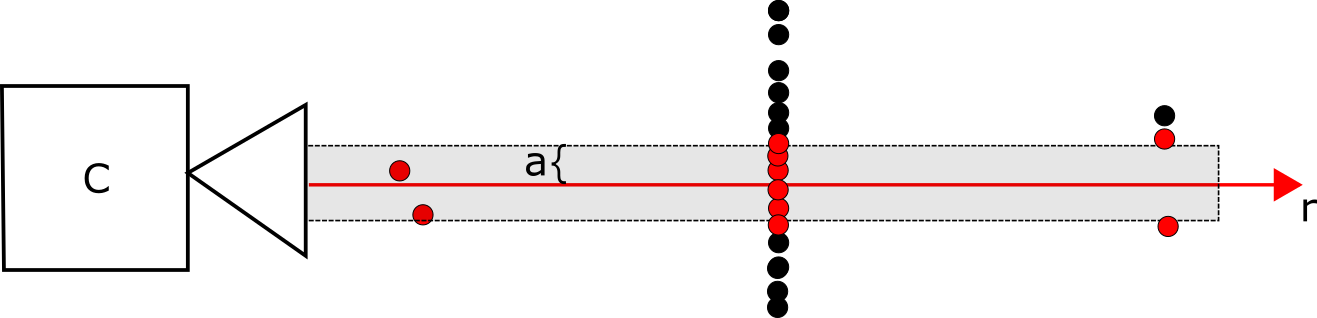
\includegraphics[width=\textwidth]{img/shootRay}
    \caption{Piste valitaan pilvestä ampumalla säde $r$ kamerasta $C$ maisemaan. $a$- säteisen lieriön sisäpuolella olevista, punaisella merkatuista pisteistä jokin on käyttäjän haluama piste.} 
    \label{img:ray}
\end{figure}

Jotta voitaisiin välttää väärien pisteiden valitseminen vahingossa, kannattaa säteen läheltä ensin kerätä useampi potentiaalinen piste, joista lopullinen valintapiste valitaan. Kuvassa \ref{img:ray} on esitetty kamerasta $C$ lähtevä säde $r$, jonka ympärillä on $a$-säteinen lieriö. Kaikki lieriön sisäpuolella olevat pisteet valitaan jatkokäsiteltäväksi. Yksinkertainen, mutta käytännössä toimivaksi todettu tapa hylätä ei-toivotut pisteet potentiaalisisten pisteiden joukosta on järjestää pisteet niiden kamerasta katsotun etäisyyden perusteella ja jättää pois lähin ja kauimmaisin kolmasosa. Jäljelle jääneistä pisteistä valitaan se, joka on lähinnä sädettä.

Scheiblauer esittää väitöskirjassaan sisäkkäisille muokattaville oktettipuille erityistä tietorakennetta valittujen pisteiden käsittelyyn. Scheiblauer valitsee pisteitä puusta laatikkovalitsimella tai kolmiulotteisella siveltimellä \engl{volumetric brush}, ja lisää ne erityiseen valintaoktettipuuhun \engl{selection octree}. Kun halutut pisteet on valittu, kuvaa valintaoktettipuu valittujen pisteiden asuttamaa avaruuden osaa. Valintaoktettipuuta käytetään esimerkiksi pisteiden piilottamiseen näkymästä. \cite{scheiblauer} Pisteitä renderöitäessä tarkastetaan, osuuko sen sijainti valintaoktettipuun solmuihin ja päätetään sen perusteella, hylätäänkö piste vai ei. Tämän tutkielman yhteydessä valintaoktettipuuta ei toteutettu, sillä piilotettavien ja renderöitävien pisteiden erottelu onnistui tarpeeksi nopeasti määrittämällä valintalaatikoita ja tarkastamalla, kuuluuko renderöitävä puun solmu osittain tai kokonaan valintalaatikkoon. 
